\documentclass[12pt,fullpage,letterpaper]{article}

\newenvironment{proof}{\noindent{\bf Proof:}}{\qed\bigskip}

\newtheorem{theorem}{Theorem}
\newtheorem{corollary}{Corollary}
\newtheorem{lemma}{Lemma} 
\newtheorem{claim}{Claim}
\newtheorem{fact}{Fact}
\newtheorem{definition}{Definition}
\newtheorem{assumption}{Assumption}
\newtheorem{observation}{Observation}
\newtheorem{example}{Example}
\newcommand{\qed}{\rule{7pt}{7pt}}

\newcommand{\assignment}[4]{
\thispagestyle{plain} 
\newpage
\setcounter{page}{1}
\noindent
\begin{center}
\framebox{ \vbox{ \hbox to 6.28in
{\bf CS446: Machine Learning \hfill #1}
\vspace{4mm}
\hbox to 6.28in
{\hspace{2.5in}\large\mbox{Problem Set #2}}
\vspace{4mm}
\hbox to 6.28in
{{\it Handed Out: #3 \hfill Due: #4}}
}}
\end{center}
}


\newcommand{\handout}[3]{
\thispagestyle{plain} 
\newpage
\setcounter{page}{1}
\noindent
\begin{center}
\framebox{ \vbox{ \hbox to 6.28in
{\bf CS446: Machine Learning \hfill #1}
\vspace{4mm}
\hbox to 6.28in
{\hspace{2.5in}\large\mbox{#2}}
\vspace{4mm}
\hbox to 6.28in
{{\it Handed Out: #3 \hfill Name (NetID): \rule[-2pt]{4cm}{0.1pt} }}
}}
\end{center}
}


\newcommand{\assgsoln}[4]{
\thispagestyle{plain} 
\newpage
\setcounter{page}{1}
\noindent
\begin{center}
\framebox{ \vbox{ \hbox to 6.28in
{\bf CS446: Machine Learning \hfill #1}
\vspace{4mm}
\hbox to 6.28in
{\hspace{2.5in}\large\mbox{Problem Set #2 Solutions}}
\vspace{4mm}
\hbox to 6.28in
{{\it Handed Out: #3 \hfill Handed In: #4}}
}}
\end{center}
}


\newcommand{\solution}[4]{
\thispagestyle{plain} 
\newpage
\setcounter{page}{1}
\noindent
\begin{center}
\framebox{ \vbox{ \hbox to 6.28in
{\bf CS446: Machine Learning \hfill #4}
\vspace{4mm}
\hbox to 6.28in
{\hspace{2.5in}\large\mbox{Problem Set #3}}
\vspace{4mm}
\hbox to 6.28in
{#1 \hfill {\it Handed In: #2}}
}}
\end{center}
\markright{#1}
}


\newenvironment{algorithm}
{\begin{center}
\begin{tabular}{|l|}
\hline
\begin{minipage}{1in}
\begin{tabbing}
\quad\=\qquad\=\qquad\=\qquad\=\qquad\=\qquad\=\qquad\=\kill}
{\end{tabbing}
\end{minipage} \\
\hline
\end{tabular}
\end{center}}

\def\Comment#1{\textsf{\textsl{$\langle\!\langle$#1\/$\rangle\!\rangle$}}}


\usepackage{amsmath}
\usepackage{algorithm}% http://ctan.org/pkg/algorithm
\usepackage{algpseudocode}% http://ctan.org/pkg/algorithmicx
\usepackage{graphicx}
\usepackage{listings}
\graphicspath{ {.} }

\DeclareMathOperator{\proj}{proj}
\newcommand{\vctproj}[2][]{\proj_{\vec{#1}}\vec{#2}}

\oddsidemargin 0in
\evensidemargin 0in
\textwidth 6.5in
\topmargin -0.5in
\textheight 9.0in

\begin{document}

\solution{Bangqi Wang}{\today}{3}{Spring 2017}
% Fill in the above, for example, as follows:
% \solution{Joe Smith}{\today}{1}{Fall 2012}

\pagestyle{myheadings}  % Leave this command alone

\begin{enumerate}
\item[1.] Answer to problem 1
	\begin{enumerate}
	\item[a.] Run the tuning procedure and record the optimal parameters.\\
		\begin{center}
		    \begin{tabular}{|p{4.0cm}|p{2.2cm}|p{2.5cm}|p{2.5cm}|p{2.5cm}|}
		      \hline
		      Algorithm               &  Parameters & Dataset n=500 & Dataset n=1000 \\\hline\hline
		      Perceptron              &  -          & -             & -              \\\hline
		      Perceptron w/margin     &  lr         & 0.005         & 0.005          \\\hline
		      Winnow                  &  alpha      & 1.1           & 1.1            \\\hline
		      Winnow w/margin         &  alpha, lr  & 1.1, 2.0      & 1.1, 0.3       \\\hline
		      AdaGrad                 &  lr         & 0.25          & 0.25           \\\hline
		    \end{tabular}
		\end{center}
		.\\
	\item[b.] Plot the cumulative number of mistakes made.\\
		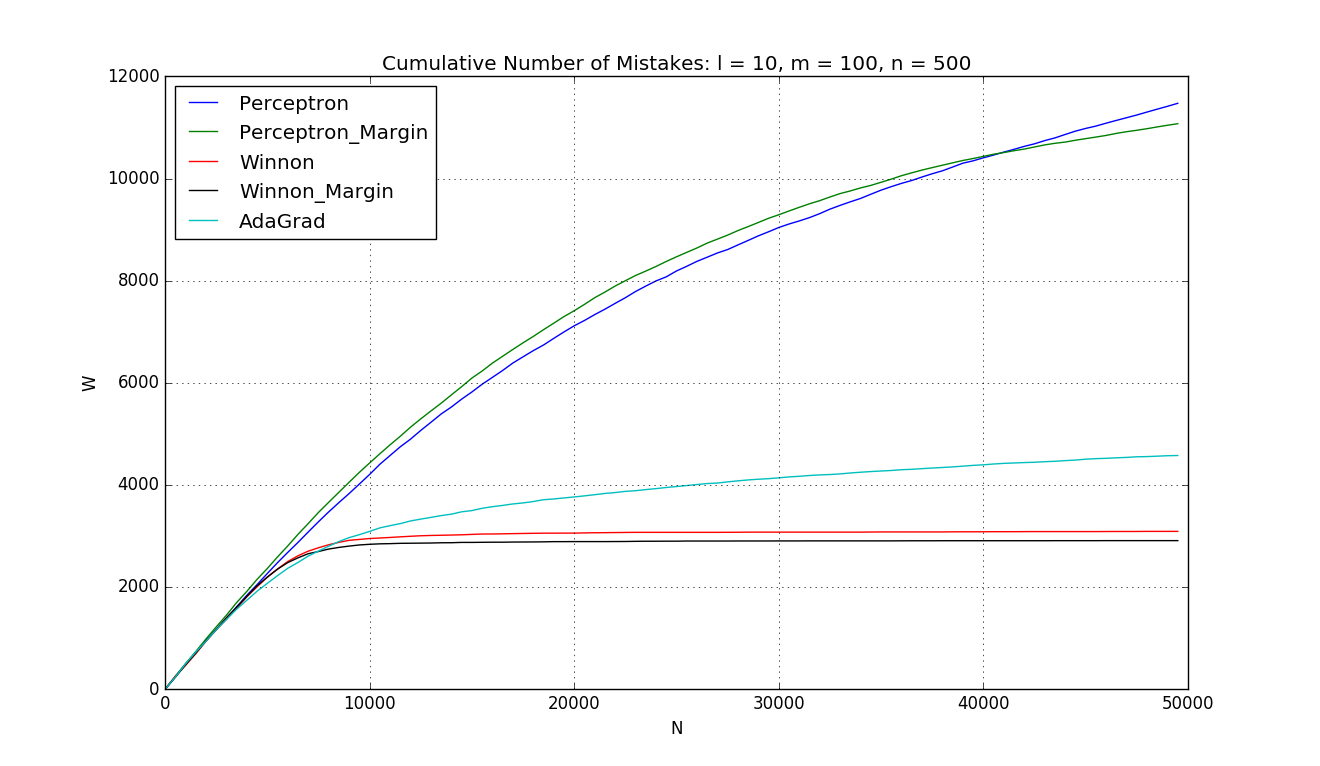
\includegraphics[width=15cm]{figure_1} \\
		In this plot, \textbf{perceptron} made most mistakes; \textbf{perceptron with margin} made a little less after long runing; \textbf{winnon with margin} made least mistakes; \textbf{winnon} made a little more; \textbf{adagrad} made mistakes in between.\\ 
		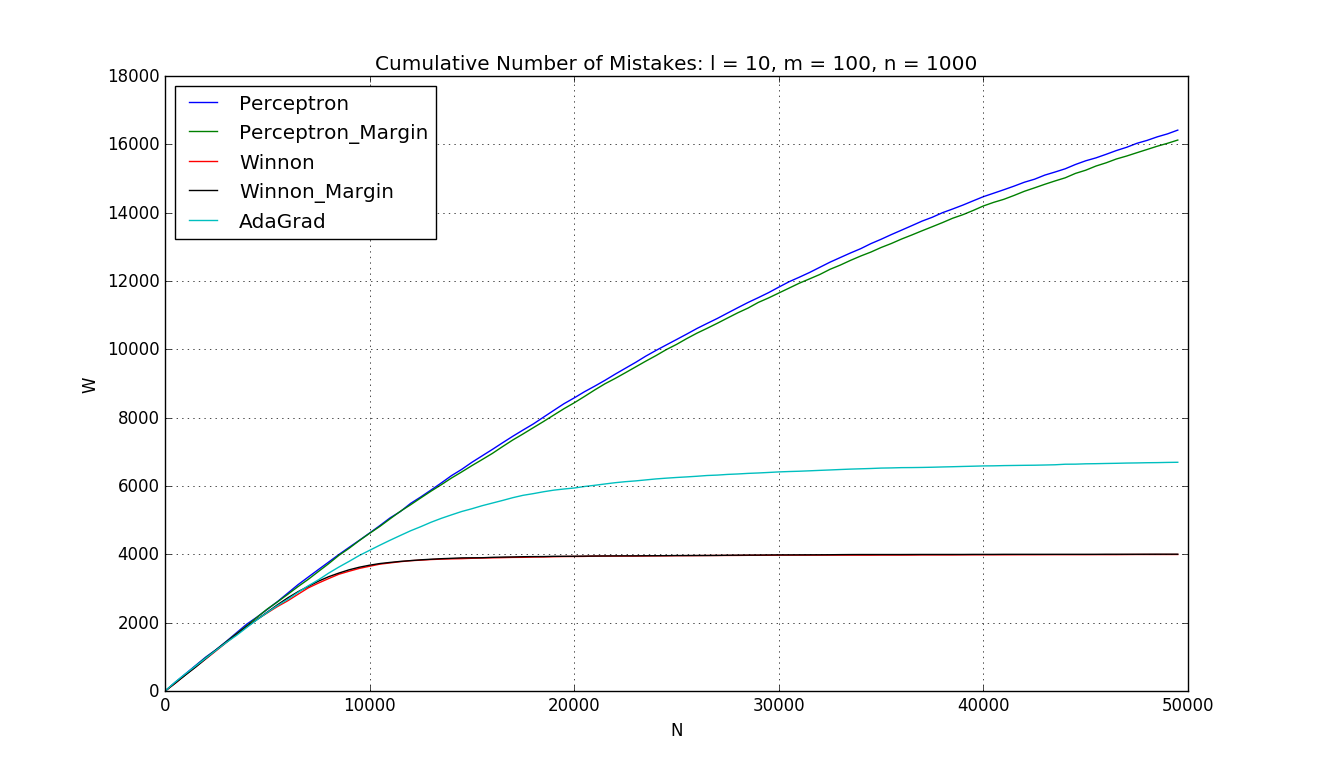
\includegraphics[width=15cm]{figure_2} \\
		In this plot, the overall tendency is almost the same, except that the number is larger. The number of mistakes made by \textbf{perceptron} increases from around $12000$ to around $16000$. The number of mistakes made by \textbf{adagrad} increases from around $5000$ to around $7000$. The number of mistakes made by \textbf{winnon} increases from around $3000$ to around $4000$. The amounts of increase are different.
	\item[c.] According to the plots above, we can verify that \textbf{perceptron} made $O(n)$ mistakes, and \textbf{winnon} made $O(mlogn)$ mistakes. Since $n$ is much larger than $m$, \textbf{winnon} made less mistakes. \textbf{adagrad} is a modified version of \textbf{perceptron}, which encourages the model to exploit infrequent features, made less mistakes when $l$ is far less than $m$.\\
	\end{enumerate}
\item[2.] Answer to problem 2
	\begin{enumerate}
	\item[a.] Record the chosen parameters.\\
		\begin{center}
	    	\begin{tabular}{|p{4.0cm}|p{1.5cm}|p{1.3cm}|p{1.3cm}|p{1.3cm}|p{1.3cm}|p{1.3cm}|}
		    	\hline
		    	Algorithm           &  Params.   & n=40     & n=80     & n=120    & n=160    & n=200    \\\hline\hline
		    	Perceptron          &  -            & -        & -        & -        & -        & -        \\\hline
		    	Perceptron w/margin &  lr           & 0.25     & 0.03     & 0.03     & 0.03     & 0.03     \\\hline
		    	Winnow              &  $\alpha$        & 1.1      & 1.1      & 1.1      & 1.1      & 1.1      \\\hline
		    	Winnow w/margin     &  $\alpha$, $\gamma$ & 1.1, 2.0 & 1.1, 2.0 & 1.1, 2.0 & 1.1, 2.0 & 1.1, 2.0 \\\hline
		    	AdaGrad             &  lr           & 1.5      & 1.5      & 1.5      & 1.5      & 1.5      \\\hline
		    \end{tabular}
		 \end{center}
		 .\\\\
	\item[b.] Plot the cumulative number of mistakes made.\\
		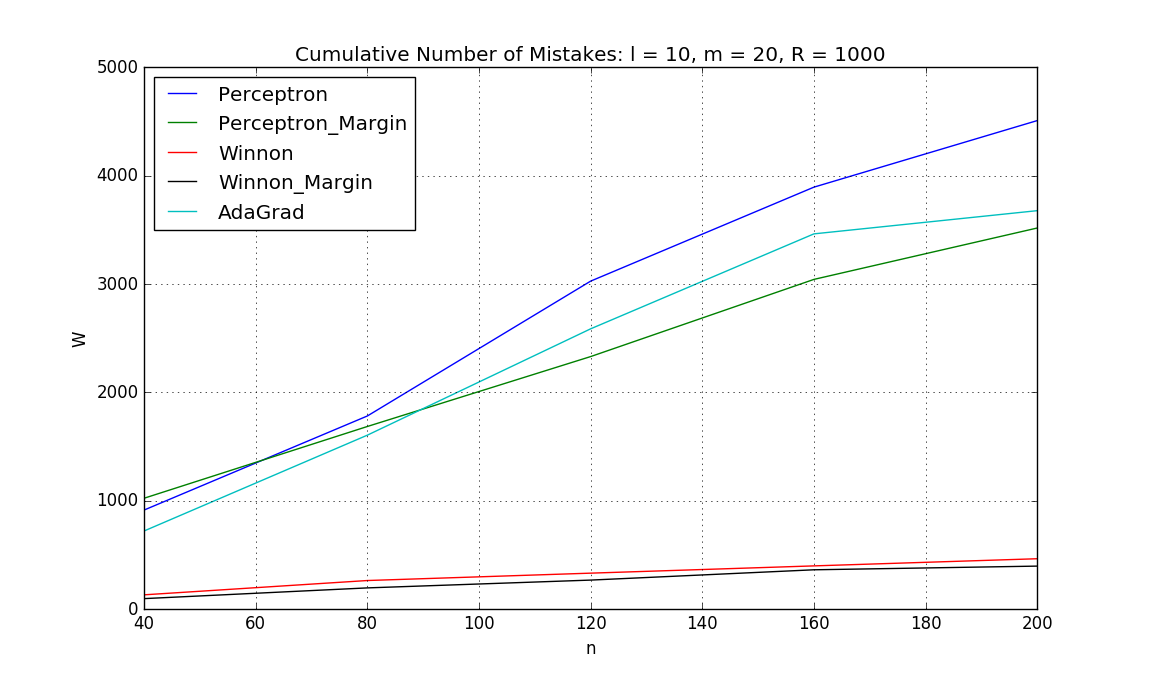
\includegraphics[width=15cm]{figure_3} 
	\item[c.] In the plot above, \textbf{perceptron} has worst performance; \textbf{perceptron with margin} and \textbf{adagrad} have a little better performance; \textbf{winnow} and \textbf{winnon with margin} have much better performance, and \textbf{winnon with margin} is little better than \textbf{winnon}. The data with large $n$ are sparser and therefore need more rounds to achieve high accuracy.\\
	\end{enumerate}
\item[3.] Answer to problem 3
	\begin{enumerate}
	\item[a.] Tuned parameters and resulting accuracy.
	\begin{center}
	 	\begin{tabular}{|p{4.0cm}|p{1.2cm}|p{1.5cm}|p{1.2cm}|p{1.5cm}|p{1.2cm}|p{1.6cm}|}
		\hline
		 Algorithm      &  \multicolumn{2}{c|}{m=100} & \multicolumn{2}{c|}{m=500} & \multicolumn{2}{c|}{m=1000}\\\hline\hline
 							 &acc.     & params.                       & acc.    & params.                        & acc.    & params.    \\\hline
		 Perceptron          & 82.03\% & -                             & 62.08\% & -                              & 75.57\% & -          \\\hline
		 Perceptron w/margin & 99.83\% & lr: 0.001                     & 97.96\% & lr: 0.005                      & 82.41\% & lr: 0.25   \\\hline
		 Winnow              & 97.72\% & $\alpha$: 1.1                 & 89.09\% & $\alpha$: 1.01                 & 71.43\% & $\alpha$: 1.1 \\\hline
		 Winnow w/margin     & 96.03\% & $\alpha$: 1.1, $\gamma$: 0.04 & 92.41\% & $\alpha$: 1.1, $\gamma$: 0.001 & 80.89\% & $\alpha$: 1.005, $\gamma$: 2.0 \\\hline
		 AdaGrad             & 99.96\% & lr: 0.03                      & 99.31\% & lr: 1.5                        & 83.59\% & lr: 0.25   \\\hline
		\end{tabular}
	\end{center}
	.\\
	\item[b.] From table above, we know that algorithms get lower accuracy in dataset with larger $m$. \textbf{adagrad} has highest accuracy; \textbf{perceptron with margin} has second highest accuracy; \textbf{winnon with margin} has third highest accuracy; \textbf{winnon} is forth, and \textbf{perceptron} is the last one. The algorithms with margin can achieve higher accuracy than original algorithms. According to plots in question 1 and 2, \textbf{winnon} made far less mistakes but \textbf{adagrad} has higher accuracy.\\
	\end{enumerate}
\item[4.] Answer to bonus problem
	\begin{enumerate}
	\item[a.] Plot the misclassification error.\\
	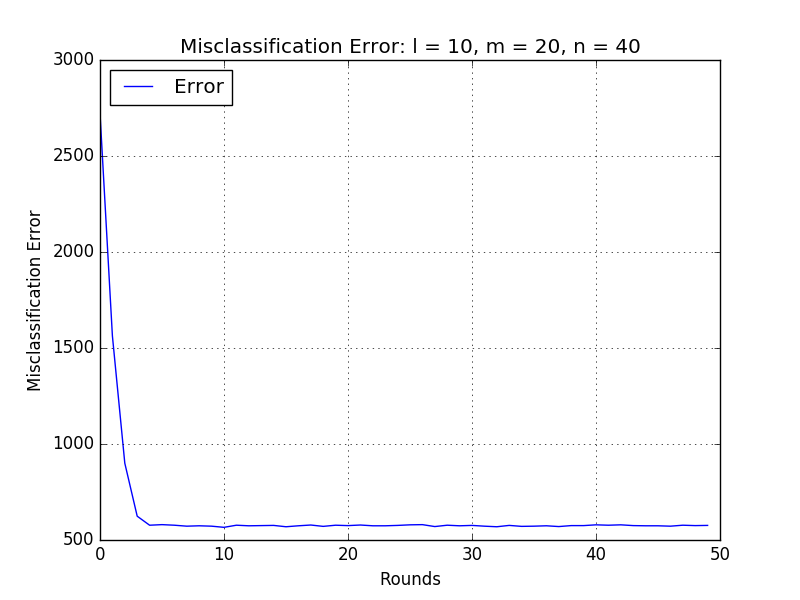
\includegraphics[width=12cm]{figure_4}
	\item[b.] Plot the hinge loss.\\
	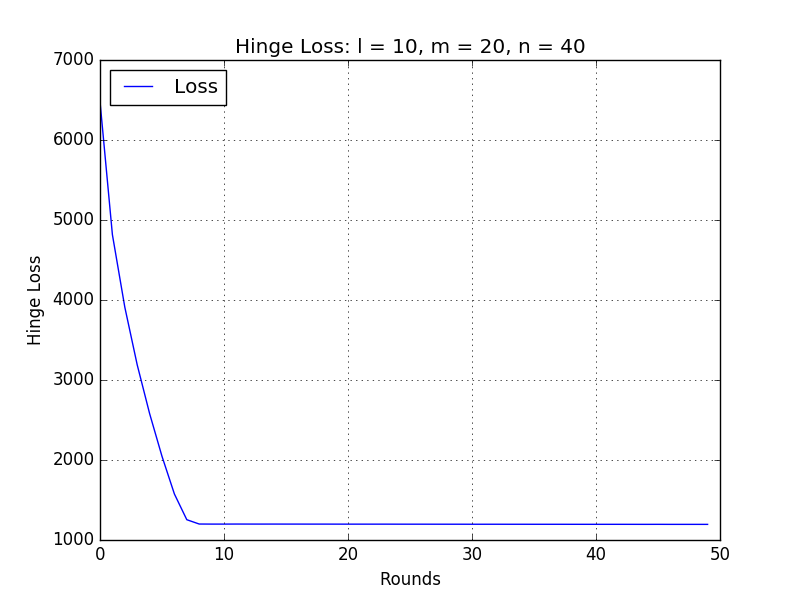
\includegraphics[width=12cm]{figure_5}\\\\
	\item[c.] Plot the misclassification error after first 10 rounds.\\
	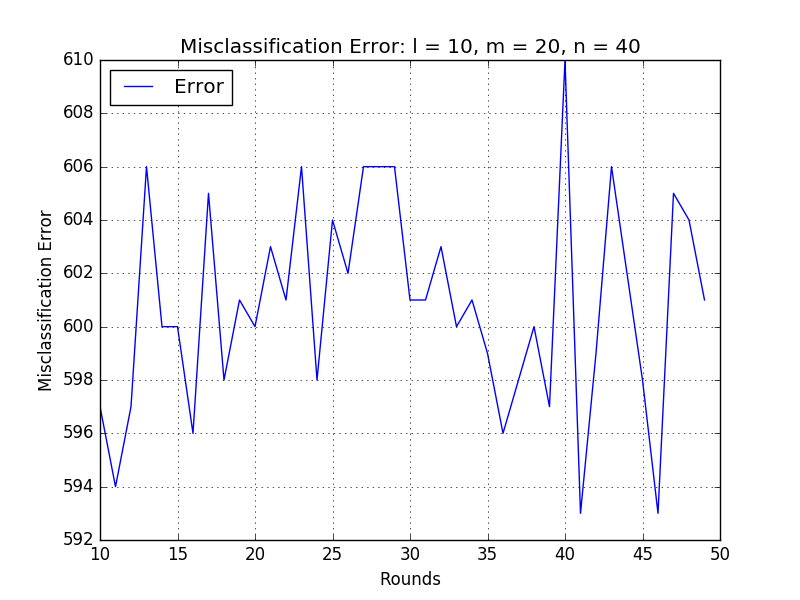
\includegraphics[width=12cm]{figure_6}
	\item[d.] Plot the hinge loss after first 10 rounds.\\
	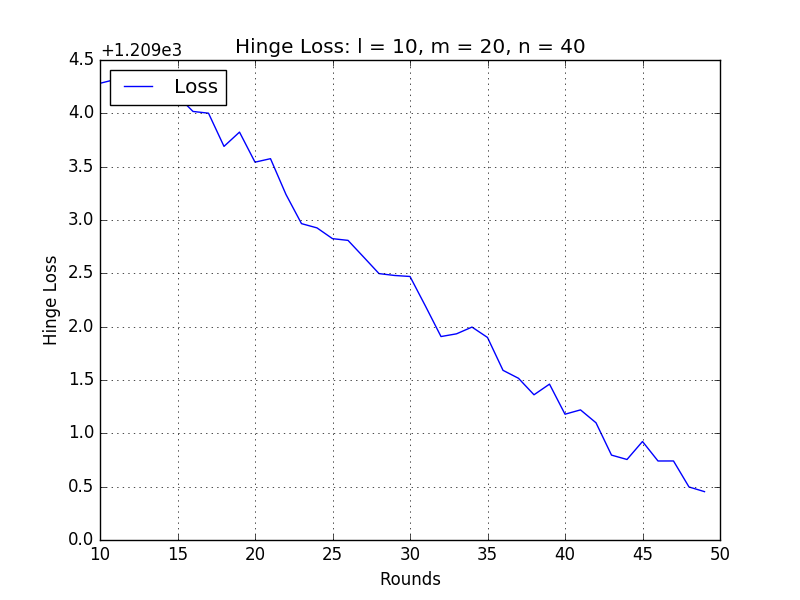
\includegraphics[width=12cm]{figure_7}
	\item[e.] From plots above, we know that \textbf{error} drops much faster than \textbf{loss} does. However, after first several rounds, \textbf{error} starts to vibrate around a certain range, but \textbf{loss} keeps decreasing.
	\end{enumerate}
\end{enumerate}

\end{document}

